\chapter{State of the Art}

\label{ch:State}

\section{Markov Chain}

As shown in \cref{fig:fig2.1}, Markov Chain is involved in Bayesian inference calculation and can therefore reduce the analysis time and provide reasonable posterior results.


  \begin{figure}[htbp]
      \centering
       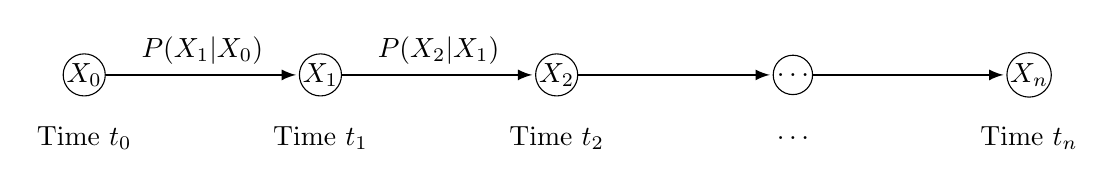
\begin{tikzpicture}[
              node distance=3cm,
              state/.style={circle, draw, fill=white, inner sep=0pt, minimum size=5mm},
              arrow/.style={->, >=latex, shorten >=1pt, thick}
            ]
              % Define state nodes
              \node[state] (X0) {$X_0$};
              \node[state, right of=X0] (X1) {$X_1$};
              \node[state, right of=X1] (X2) {$X_2$};
              \node[state, right of=X2] (Xdots) {$\dots$};
              \node[state, right of=Xdots] (Xn) {$X_n$};
            
              % Draw arrows
              \draw[arrow] (X0) -- node[above] {$P(X_1|X_0)$} (X1);
              \draw[arrow] (X1) -- node[above] {$P(X_2|X_1)$} (X2);
              \draw[arrow] (X2) -- node[above] {} (Xdots);
              \draw[arrow] (Xdots) -- node[above] {} (Xn);
            
              % Add time labels
              \node[below of=X0, node distance=0.8cm] (T0) {Time $t_0$};
              \node[below of=X1, node distance=0.8cm] (T1) {Time $t_1$};
              \node[below of=X2, node distance=0.8cm] (T2) {Time $t_2$};
              \node[below of=Xdots, node distance=0.8cm] (Tdots) {$\dots$};
              \node[below of=Xn, node distance=0.8cm] (Tn) {Time $t_n$};
            \end{tikzpicture}
              
      \caption{Markov Chain process}
      \label{fig:fig2.1}
  \end{figure}

  Markov Chain has two main features:
  \begin{itemize}
      \item State transition of Markov chains depends only on the current state, thus simplifying the modeling process
      \item Given the current state, a state transition probability distribution can be used to infer the likelihood of the next state

  \end{itemize}

  Thus, the properties of Markov Chain will bring two advantages: 

  \begin{itemize}
      \item Adapt to more complex models (with increasing soil parameters)
      \item Iterative updating of parameter estimates because of Markov Chain’s property (enables  updating the priors through Bayesian inference in stage)

  \end{itemize}


  \section{Partially observed Markov decision process (POMDP)}

As shown in \cref{fig:fig2.2}, based on Markov Chain, with introducing Rewards and Actions, it can form the basis of Partially observed Markov decision process.


\begin{figure}[htbp]
    \centering
    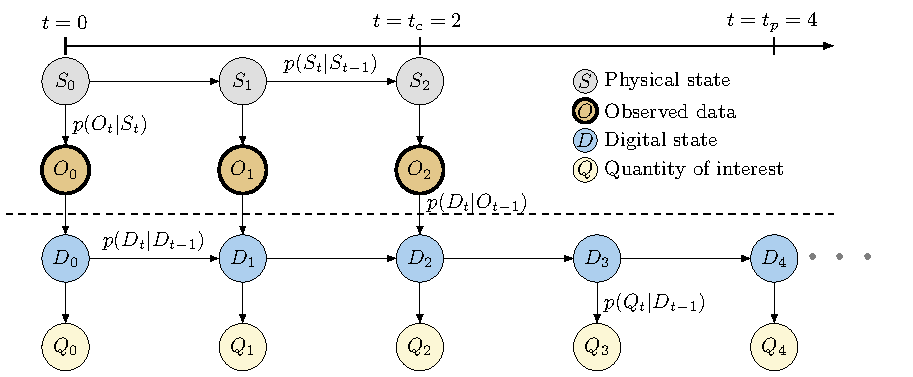
\includegraphics[width = 140mm]{Figures/figure3.pdf}
    \caption{Untrained strength profile at Cowden \protect\cite{kapteyn2021}}
    \label{fig:fig2.2}
\end{figure}


\section{Digital Twin}

Generally, Digital Twin can be divided into two main parts, including (1) calibration and assimilation (2) Prediction, as shown in \cref{equation 2.1}  and \cref{equation 2.2}.

\begin{equation}
\begin{aligned}
& p(D_{0},...,D_{t_{c}},Q_{0},...,Q_{t_{c}},R_{0},...,R_{t_{c}}|o_{0},...,o_{t_{c}},u_{0},...,u_{t_{c}}) \\
& = \prod_{t=0}^{t_{c}}[\phi_{t}^{update}\phi_{t}^{QoI}\phi_{t}^{evaluation}] \label{equation 2.1}
\end{aligned}
\end{equation}


\begin{equation}
\begin{aligned}
    & p(D_{0},...,D_{t_{p}},Q_{0},...,Q_{t_{p}},R_{0},...,R_{t_{p}},U_{t_{c}+1},...,U_{t_{p}}|o_{0},...,o_{t_{c}},u_{0},...,u_{t_{c}}) \\
    & \propto \prod_{t=0}^{t_{p}}[\phi_{t}^{dynamics}\phi_{t}^{QoI}\phi_{t}^{evaluation}] \prod_{t=0}^{t_{c}}\phi_{t}^{assimilation} \prod_{t=t_{c}+1}^{t_{p}}\phi_{t}^{control} \label{equation 2.2}
\end{aligned}
\end{equation}